\chapter{Réalisation}
	
\section*{Introduction}
   Après avoir achevé la partie de conception, nous allons entamer dans ce chapitre l’implémentation et la réalisation de notre système en présentant l'architecture et les interfaces de notre application.

\section{Les outils utiliséss}
Dans cette section, nous allons identifier les différentes technologies utilisées dans notre application.


\subsection{Node.js}


\subsection{HTML 5 / CSS 3}
HTML est considéré comme un langage de balisage qui a pour but d'organiser et de structurer des pages web et CSS qui est le complémentaire de HTML permet de définir des styles de ces pages \cite{HTMLCSS}.\\
Les versions 3 et 5 ont été choisies et utilisées respectivement pour CSS et HTML dans le but de créer des interfaces graphiques pour notre application.   
\subsection{JavaScript}                 
JavaScript est le langage de programmation du HTML et du Web. Il est utilisé dans les pages web interactives \cite{JavaScript}.                
\subsection{BootStrap}
Bootstrap est le framework HTML, CSS et JavaScript le plus populaire pour le développement de sites web réactifs et mobiles \cite{BootStrap}.\\
La version 4 de cette technologie a été choisie et qui a été utilisée pour améliorer et fournir une interface conviviale.
\newpage
\subsection{Angular 4}
Angular 4 est un framework javascript qui facilite la création d'applications sur le web. Il combine les modèles déclaratifs, l'injection de dépendance et les meilleures pratiques intégrées pour résoudre les problèmes de développement \cite{Angular}.


\subsection{MongoDb}
MongoDB stocke des données dans des documents flexibles de type JSON, ce qui signifie que les champs peuvent varier d'un document à l'autre et que la structure des données peut être modifiée au fil du temps \cite{MongoDb}. La version 3 de Mongodb a été choisie dans l'objectif de gérer de grandes quantités de données.

\section{Environnement matériel}
Pour élaborer ce projet, un micro-ordinateur portable LENOVO Z510 a été utilisé. Il est exploité sous le système d’exploitation Windows 8.1 et il possède les caractéristiques suivantes :
\begin{itemize}

    \item Processeur Intel CORE i7-4702 MQ, 2.20 GHz;
    
   \item  Mémoire vive «RAM» d’une capacité de 8 GO;

   \item  Ecran de 15,6 (15,6 pouces);

 \item	  Disque dur d’une capacité de 1 TO.
\end{itemize}
\newpage
\section{Architecture de l'application}
La figure \ref{fig:architecture de projet} ci-après expose l'architecture de notre application. En effet, l'utilisateur interagit avec la couche de présentation de notre application développée avec Angular version (4) qui communique avec H2o.ai.
%L’objectif de notre projet est de développer une application en utilisant comme technologies Angular 4 de côté Client et Node.js de côté Serveur %.
De côté Serveur, le choix a été effectué sur Express.js pour interagir avec la couche de présentation de notre application et Mongoose pour communiquer avec la base de données MongoDB version (3.4.6).\\
Notre application permet aussi de récupérer des informations de la plateforme H2o.ai pour construire des modèles, effectuer des prédictions et récupérer des résultats pour les stocker dans MongoDB et les afficher dans notre application.\\
    \begin{figure}[htpb]
    \centering
    \fcolorbox{black}{white}{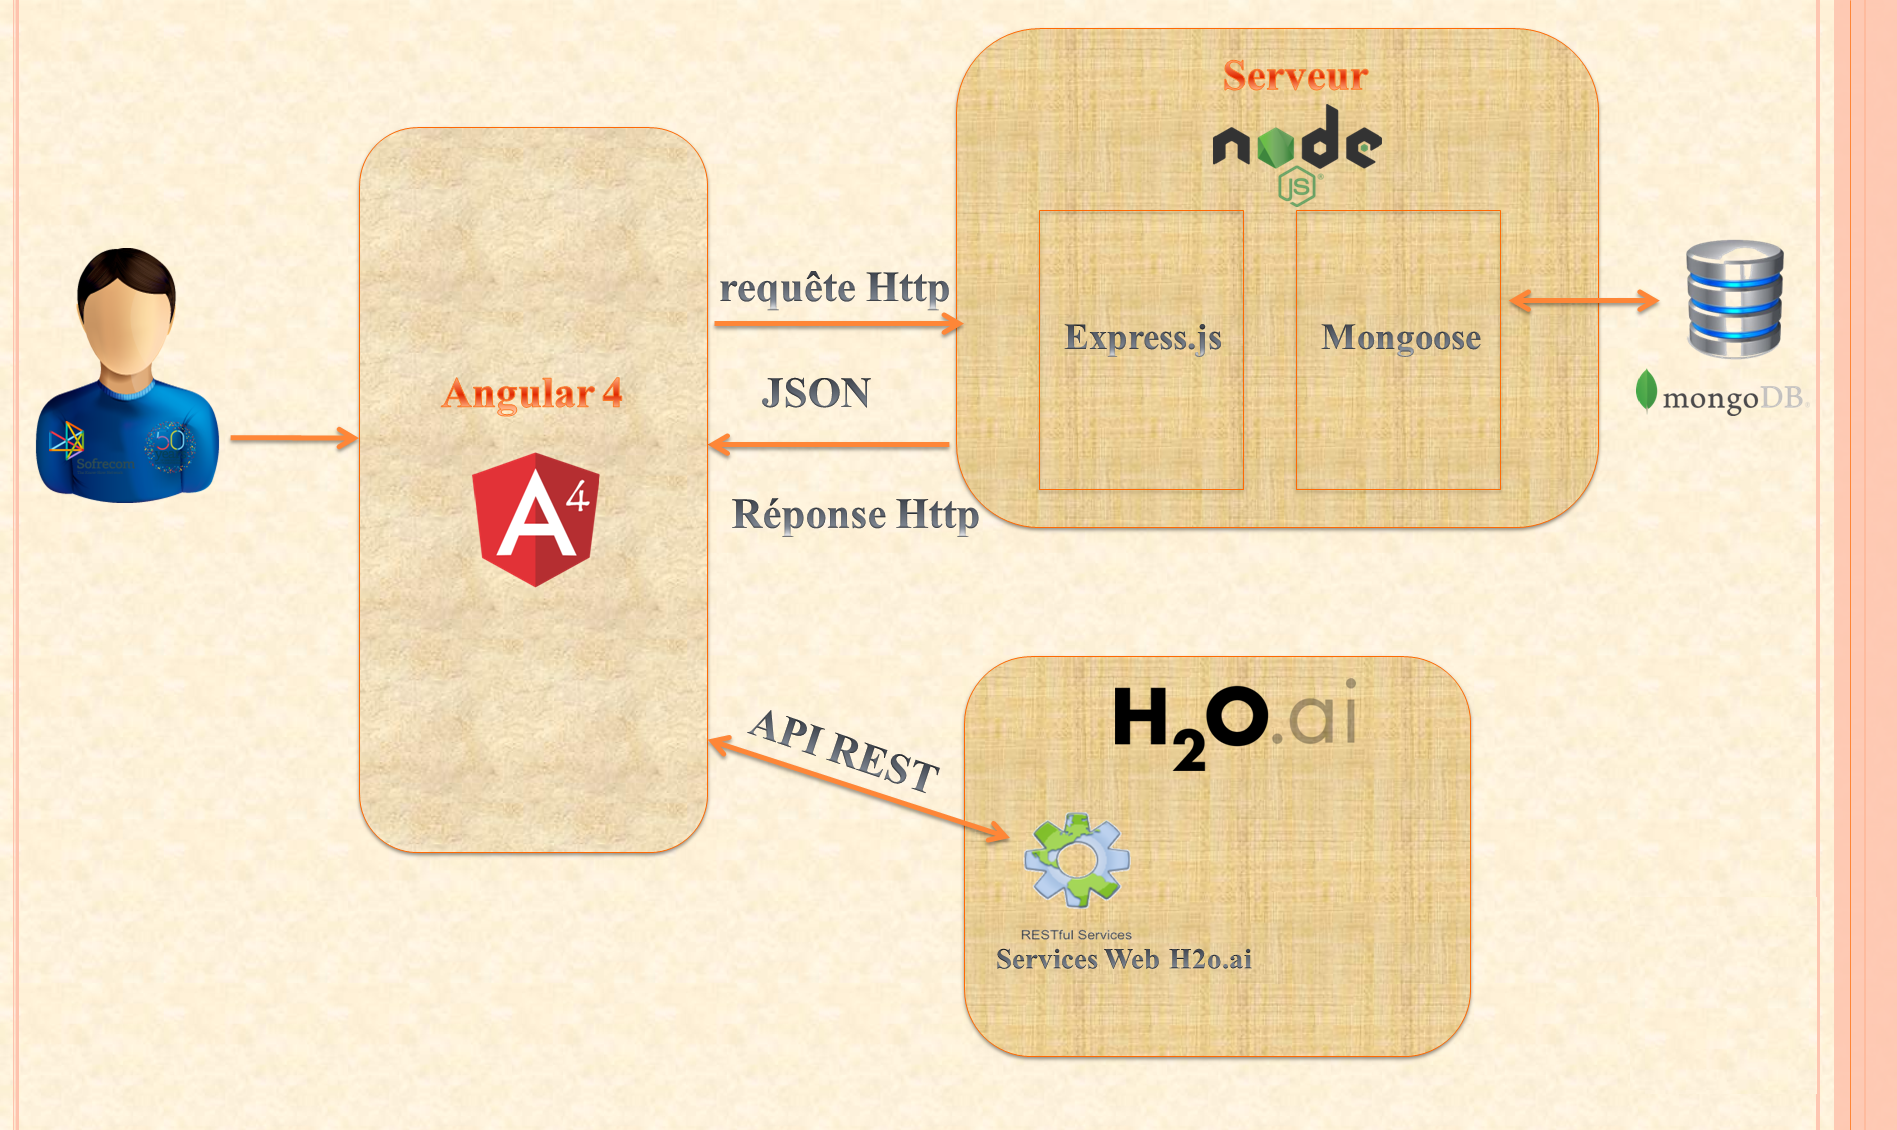
\includegraphics[width=1\linewidth]{img/architectureApp.png}}
    \caption{L'architecture de projet}
    \label{fig:architecture de projet}
    \end{figure}
    \newpage
\section{Les interfaces graphiques de l’application}
Dans cette section, nous allons exposer les différentes interfaces de notre application.\\
Nous avons choisi l’administrateur comme utilisateur vu qu’il présente à travers ces interactions la majeure partie des principales fonctionnalités de l’application.


\subsection{Authentification}
L’utilisateur doit d’abord s’authentifier pour pouvoir accéder à l’application comme la montre la figure  \ref{fig:Interfaceauthentification} ci-dessous.
    \begin{figure}[htpb]
    \centering
  \fcolorbox{black}{white}{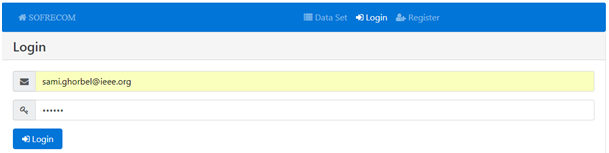
\includegraphics[width=1\linewidth]{img/realisation1.png}}
    \caption{Interface de l’authentification}
    \label{fig:Interfaceauthentification}
    \end{figure}
        \subsection{Import d'un fichier}
        L'utilisateur peut importer un fichier d'extension ".csv" comme la montre la figure \ref{fig:InterfaceImport} ci-dessous.
       \begin{figure}[htpb]
    \centering
     \fcolorbox{black}{white}{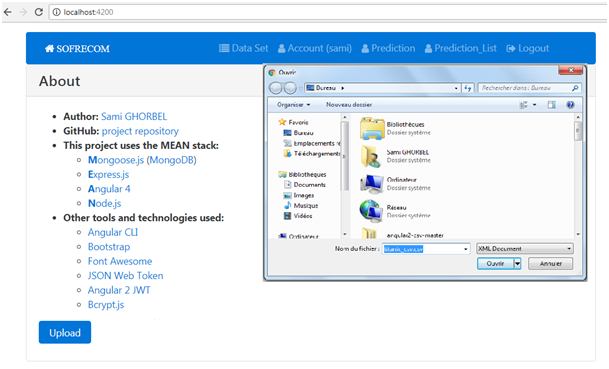
\includegraphics[width=0.85\linewidth]{img/realisation6.png}}
    \caption{Interface d'import de fichier}
    \label{fig:InterfaceImport}
    \end{figure}
    \newpage
\subsection{Prédiction}
Comme la montre la figure \ref{fig:Interface de traitement de prédiction} ci-dessous, l’utilisateur peut effectuer des prédictions selon les données et le modèle choisis. 
    \begin{figure}[htpb]
    \centering
     \fcolorbox{black}{white}{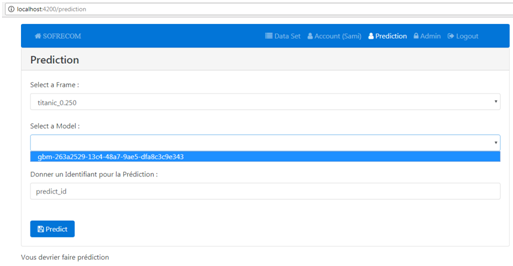
\includegraphics[width=0.85\linewidth]{img/realisation2.png}}
    \caption{Interface de traitement de prédiction}
    \label{fig:Interface de traitement de prédiction}
    \end{figure}
    \newpage
L’utilisateur peut filtrer cette prédiction et exporter cette dernière sous différents formats tels que ( xls, csv et pdf... ) comme la montre la figure     \ref{fig:Interface de résultat de prédiction} ci-dessous.
    \begin{figure}[htpb]
    \centering
    \fcolorbox{black}{white}{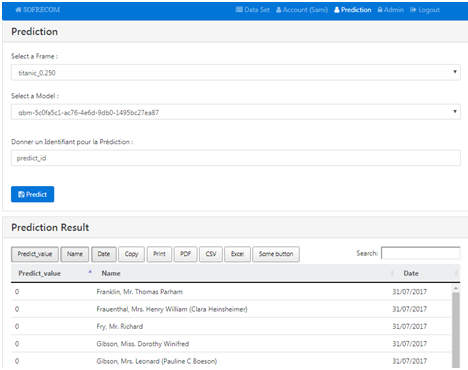
\includegraphics[width=1\linewidth]{img/realisation3.png}}
    \caption{Interface de résultat de prédiction}
    \label{fig:Interface de résultat de prédiction}
    \end{figure}   
    \newpage
\subsection{Export sous format PDF}
L’utilisateur peut exporter la liste des prédictions sous format "pdf" comme la montre la figure \ref{fig:Interfaceexport} ci-dessous.
 \begin{figure}[htpb]
    \centering
    \fcolorbox{black}{white}{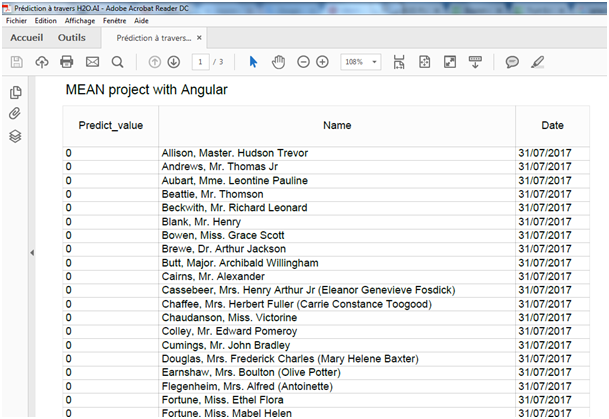
\includegraphics[width=1\linewidth]{img/realisation4.png}}
    \caption{Interface d'export sous format pdf}
    \label{fig:Interfaceexport}
    \end{figure}   
    \newpage
    
  \subsection{Consultation de la liste des prédictions}
  L’utilisateur peut consulter l’historique des prédictions de chaque employé comme la montre la figure     \ref{fig:Interfacelisteprediction}.
     \begin{figure}[htpb]
    \centering
    \fcolorbox{black}{white}{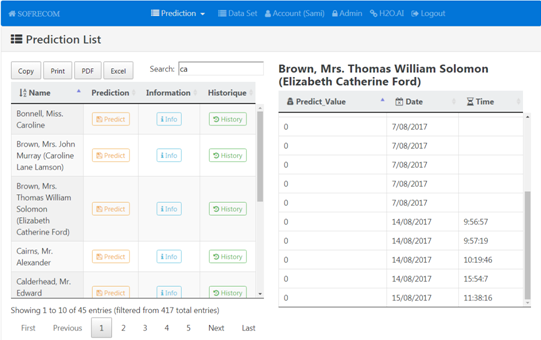
\includegraphics[width=1\linewidth]{img/realisation5.png}}
    \caption{Interface de la liste des prédictions}
    \label{fig:Interfacelisteprediction}
    \end{figure} 
\newpage
    \section{Diagramme de GANTT réel}
   Le diagramme de la figure ci-après décrit le déroulement réel des étapes du stage d'été. Pendant les dix premiers jours, les tâches préliminaires comme la documentation et l’étude  du projet ont été effectuées dans le délais prévu. Ces travaux ont été suivis par les phases de spécification des besoins, de conception, de réalisation et de tests qui sont finies comme convenu avant la date de fin du stage 31 août 2017.\\
    La rédaction de rapport a pris beaucoup de retard par rapport à ce qui a été indiquée dans le diagramme de gantt théorique.
         \begin{figure}[htpb]
\centering
  \fcolorbox{black}{white}{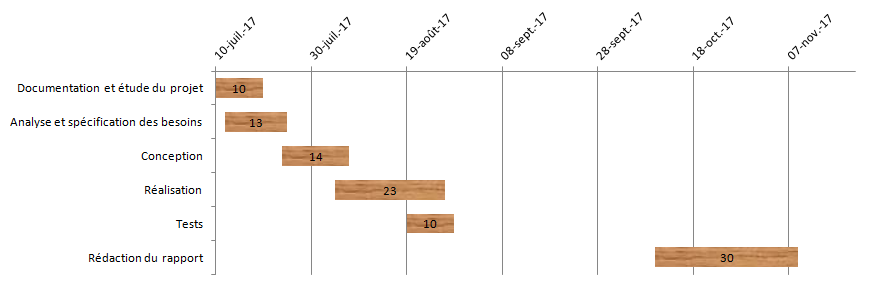
\includegraphics[width=1\linewidth]{img/gantt_reel2.png}}
\caption{Diagramme de GANTT réel}
\label{fig:Diagrammeganttreel }
\end{figure}
\section*{Conclusion}
  A travers ce chapitre, nous avons présenté la réalisation de l’application en justifiant nos choix technologiques et en représentant les différentes interfaces de l’application.